\clearpage % clearpage to makesure all tables/figures have been dumped BEFORE these
\section*{Appendix: A}
With the exception of SN1991T and SN1991bg, we provide four figures for each supernova used in this analysis. The first figure shows a blue spectrum, and possibly a red spectrum. If there is only a blue spectrum, then we applied no flux correction to the raw data, and only re-binned it and trimmed the edges off before using it in our analysis. If we show a red and a blue spectrum, then the red spectrum represents the data before flux calibration, and the blue spectrum shows the data we finally used after flux calibration.

The second figure shows a step in our flux calibration process. We fit a light curve with SALT2 and used SALT2 to generate an artificial spectrum for the supernova. We then re-binned both the supernova's spectrum and the SALT2 spectrum to 500 \AA\ bins. We compared these, and plotted a point for each bin which represents the number we'd have to multiple the data bin by to match the SALT2 bin. If a pink line is shown, then this is the function we used for the flux calibration. If no line is shown, then no flux calibration was performed.

The third figure shows the light curve fit by SALT2. The x scale of this plot is adjusted to only include the portion that SALT2 fit. While other points exist they are not included in the fit and so are not plotted.

The fourth figure shows the supernova spectrum, and the best fit using a $\chi^{2}$ fit of Hsiao's template warped with a Cardelli law. These plots were created to give an indication of the inability of a single parameter warp to account for all of a supernova's features.



\begin{figure}[p]
\centering
\includegraphics[angle=-90,width=0.8\textwidth]{./figures/spectrabeforeafter/SN1997dt_handpicked_v001_v027_before_after_spectra.ps}
\hfill
\includegraphics[angle=-90,width=0.8\textwidth]{./figures/corrections/SN1997dt_v001_correction.ps}
\hfill
\caption{SN1997dt spectrum before and after warping, as well as the correction function used to warp.}
\label{fig:SN1997dtfour1}
\end{figure}

\clearpage

\begin{figure}[p]
\centering
\includegraphics[angle=-90,width=0.8\textwidth]{./figures/ltcv/SN1997dt_v027_lightcurve.ps}
\hfill
\includegraphics[angle=-90,width=0.8\textwidth]{./figures/hsiao/SN1997dt_v001_hsiao.ps}
\hfill
\caption{SN1997dt light curve fit, as well as the best fit for Hsiao template warped using the Cardelli law to match the spectrum.}
\label{fig:SN1997dtfour2}
\end{figure}

\clearpage

\begin{figure}[p]
\centering
\includegraphics[angle=-90,width=0.8\textwidth]{./figures/spectrabeforeafter/SN1998V_handpicked_v001_v023_before_after_spectra.ps}
\hfill
\includegraphics[angle=-90,width=0.8\textwidth]{./figures/corrections/SN1998V_v001_correction.ps}
\hfill
\caption{SN1998V spectrum before and after warping, as well as the correction function used to warp.}
\label{fig:SN1998Vfour1}
\end{figure}

\clearpage

\begin{figure}[p]
\centering
\includegraphics[angle=-90,width=0.8\textwidth]{./figures/ltcv/SN1998V_v023_lightcurve.ps}
\hfill
\includegraphics[angle=-90,width=0.8\textwidth]{./figures/hsiao/SN1998V_v001_hsiao.ps}
\hfill
\caption{SN1998V light curve fit, as well as the best fit for Hsiao template warped using the Cardelli law to match the spectrum.}
\label{fig:SN1998Vfour2}
\end{figure}

\clearpage

\begin{figure}[p]
\centering
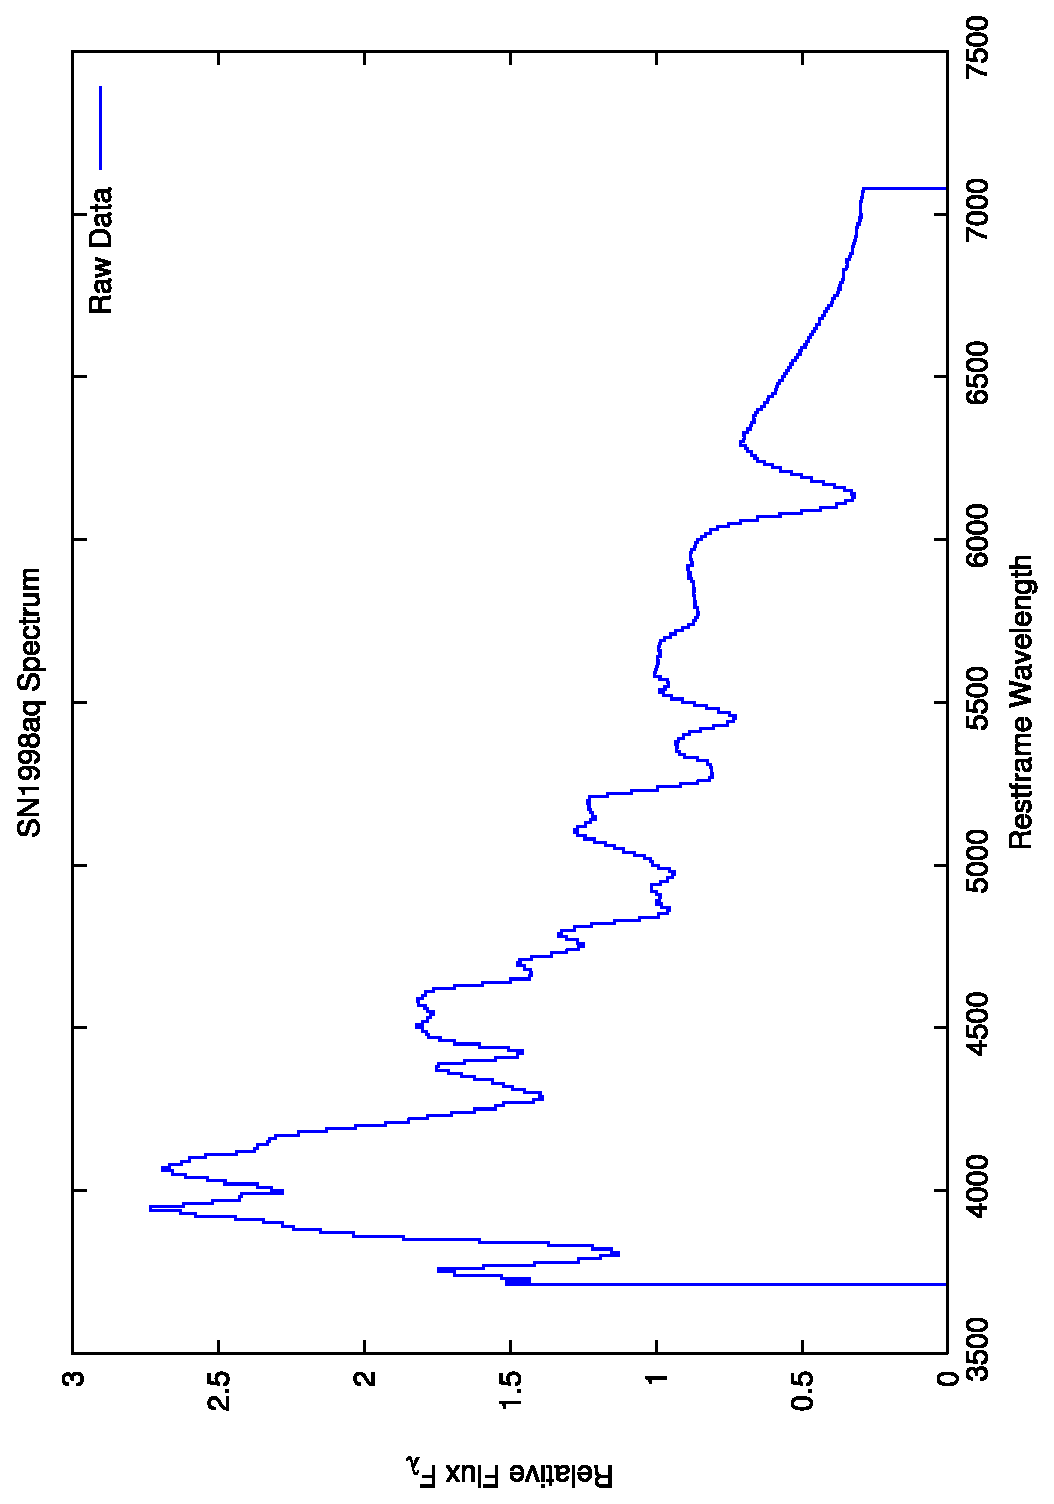
\includegraphics[angle=-90,width=0.8\textwidth]{./figures/spectrabeforeafter/SN1998aq_handpicked_v001_v027_before_after_spectra.ps}
\hfill
\includegraphics[angle=-90,width=0.8\textwidth]{./figures/corrections/SN1998aq_v001_correction.ps}
\hfill
\caption{SN1998aq spectrum before and after warping, as well as the correction function used to warp.}
\label{fig:SN1998aqfour1}
\end{figure}

\clearpage

\begin{figure}[p]
\centering
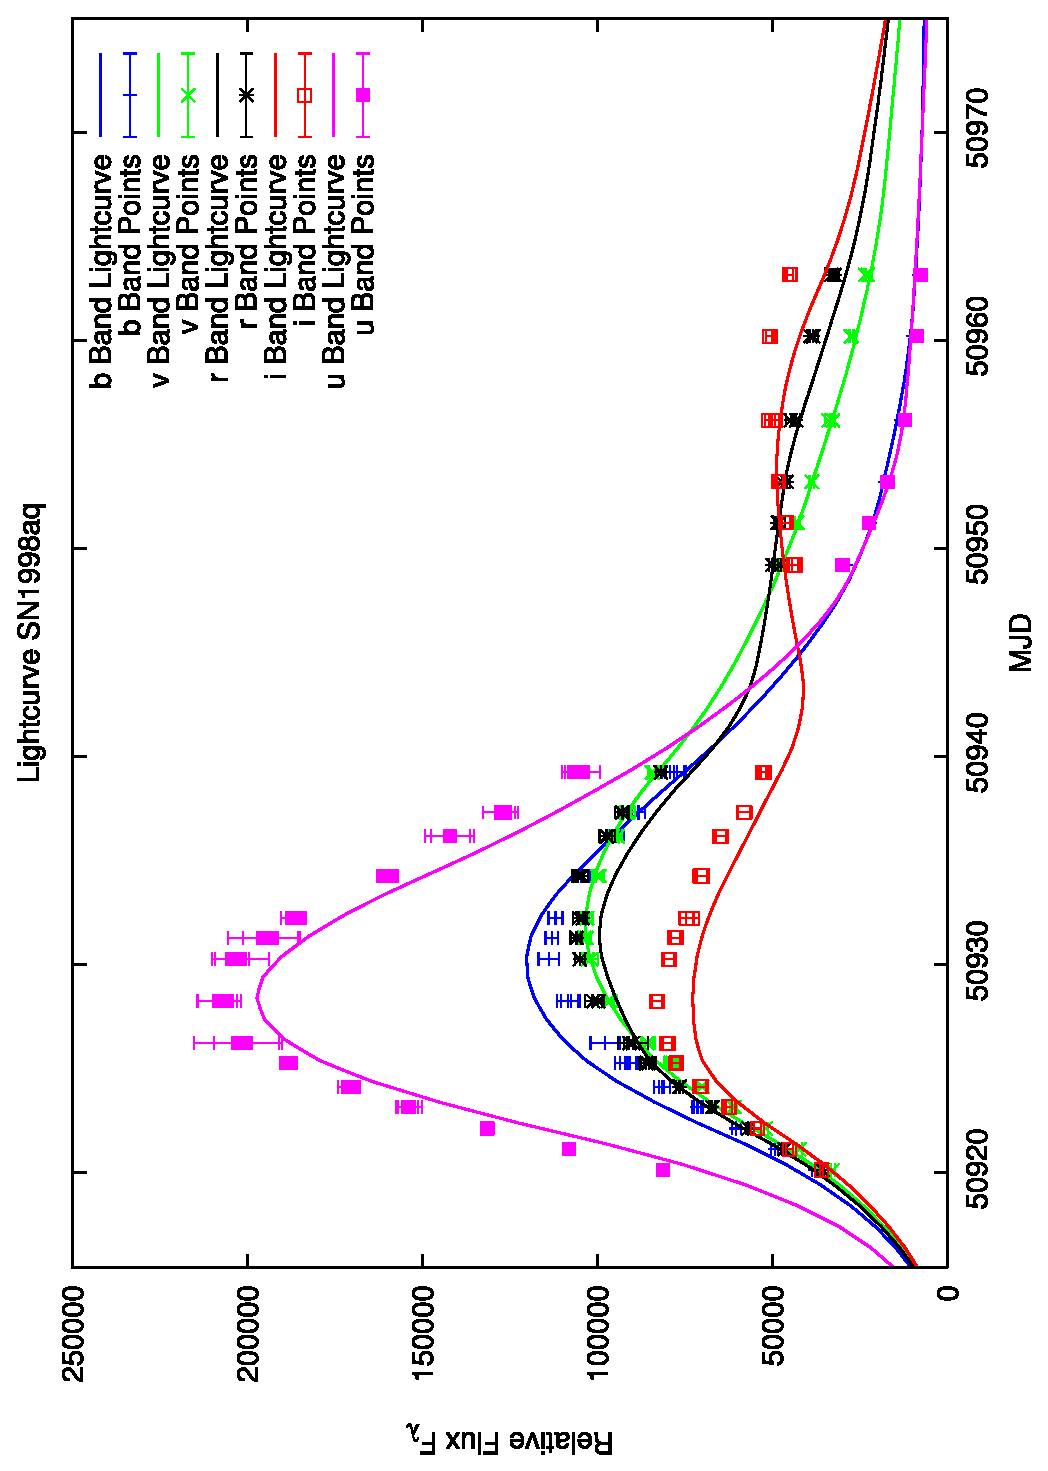
\includegraphics[angle=-90,width=0.8\textwidth]{./figures/ltcv/SN1998aq_v027_lightcurve.ps}
\hfill
\includegraphics[angle=-90,width=0.8\textwidth]{./figures/hsiao/SN1998aq_v001_hsiao.ps}
\hfill
\caption{SN1998aq light curve fit, as well as the best fit for Hsiao template warped using the Cardelli law to match the spectrum.}
\label{fig:SN1998aqfour2}
\end{figure}

\clearpage

\begin{figure}[p]
\centering
\includegraphics[angle=-90,width=0.8\textwidth]{./figures/spectrabeforeafter/SN1998bp_handpicked_v001_v027_before_after_spectra.ps}
\hfill
\includegraphics[angle=-90,width=0.8\textwidth]{./figures/corrections/SN1998bp_v001_correction.ps}
\hfill
\caption{SN1998bp spectrum before and after warping, as well as the correction function used to warp.}
\label{fig:SN1998bpfour1}
\end{figure}

\clearpage

\begin{figure}[p]
\centering
\includegraphics[angle=-90,width=0.8\textwidth]{./figures/ltcv/SN1998bp_v027_lightcurve.ps}
\hfill
\includegraphics[angle=-90,width=0.8\textwidth]{./figures/hsiao/SN1998bp_v001_hsiao.ps}
\hfill
\caption{SN1998bp light curve fit, as well as the best fit for Hsiao template warped using the Cardelli law to match the spectrum.}
\label{fig:SN1998bpfour2}
\end{figure}

\clearpage

\begin{figure}[p]
\centering
\includegraphics[angle=-90,width=0.8\textwidth]{./figures/spectrabeforeafter/SN1998de_handpicked_v001_v023_before_after_spectra.ps}
\hfill
\includegraphics[angle=-90,width=0.8\textwidth]{./figures/corrections/SN1998de_v001_correction.ps}
\hfill
\caption{SN1998de spectrum before and after warping, as well as the correction function used to warp.}
\label{fig:SN1998defour1}
\end{figure}

\clearpage

\begin{figure}[p]
\centering
\includegraphics[angle=-90,width=0.8\textwidth]{./figures/ltcv/SN1998de_v023_lightcurve.ps}
\hfill
\includegraphics[angle=-90,width=0.8\textwidth]{./figures/hsiao/SN1998de_v001_hsiao.ps}
\hfill
\caption{SN1998de light curve fit, as well as the best fit for Hsiao template warped using the Cardelli law to match the spectrum.}
\label{fig:SN1998defour2}
\end{figure}

\clearpage

\begin{figure}[p]
\centering
\includegraphics[angle=-90,width=0.8\textwidth]{./figures/spectrabeforeafter/SN1998dh_handpicked_v001_v027_before_after_spectra.ps}
\hfill
\includegraphics[angle=-90,width=0.8\textwidth]{./figures/corrections/SN1998dh_v001_correction.ps}
\hfill
\caption{SN1998dh spectrum before and after warping, as well as the correction function used to warp.}
\label{fig:SN1998dhfour1}
\end{figure}

\clearpage

\begin{figure}[p]
\centering
\includegraphics[angle=-90,width=0.8\textwidth]{./figures/ltcv/SN1998dh_v027_lightcurve.ps}
\hfill
\includegraphics[angle=-90,width=0.8\textwidth]{./figures/hsiao/SN1998dh_v001_hsiao.ps}
\hfill
\caption{SN1998dh light curve fit, as well as the best fit for Hsiao template warped using the Cardelli law to match the spectrum.}
\label{fig:SN1998dhfour2}
\end{figure}

\clearpage

\begin{figure}[p]
\centering
\includegraphics[angle=-90,width=0.8\textwidth]{./figures/spectrabeforeafter/SN1998ec_handpicked_v001_v027_before_after_spectra.ps}
\hfill
\includegraphics[angle=-90,width=0.8\textwidth]{./figures/corrections/SN1998ec_v001_correction.ps}
\hfill
\caption{SN1998ec spectrum before and after warping, as well as the correction function used to warp.}
\label{fig:SN1998ecfour1}
\end{figure}

\clearpage

\begin{figure}[p]
\centering
\includegraphics[angle=-90,width=0.8\textwidth]{./figures/ltcv/SN1998ec_v027_lightcurve.ps}
\hfill
\includegraphics[angle=-90,width=0.8\textwidth]{./figures/hsiao/SN1998ec_v001_hsiao.ps}
\hfill
\caption{SN1998ec light curve fit, as well as the best fit for Hsiao template warped using the Cardelli law to match the spectrum.}
\label{fig:SN1998ecfour2}
\end{figure}

\clearpage

\begin{figure}[p]
\centering
\includegraphics[angle=-90,width=0.8\textwidth]{./figures/spectrabeforeafter/SN1998eg_handpicked_v001_v023_before_after_spectra.ps}
\hfill
\includegraphics[angle=-90,width=0.8\textwidth]{./figures/corrections/SN1998eg_v001_correction.ps}
\hfill
\caption{SN1998eg spectrum before and after warping, as well as the correction function used to warp.}
\label{fig:SN1998egfour1}
\end{figure}

\clearpage

\begin{figure}[p]
\centering
\includegraphics[angle=-90,width=0.8\textwidth]{./figures/ltcv/SN1998eg_v023_lightcurve.ps}
\hfill
\includegraphics[angle=-90,width=0.8\textwidth]{./figures/hsiao/SN1998eg_v001_hsiao.ps}
\hfill
\caption{SN1998eg light curve fit, as well as the best fit for Hsiao template warped using the Cardelli law to match the spectrum.}
\label{fig:SN1998egfour2}
\end{figure}

\clearpage

\begin{figure}[p]
\centering
\includegraphics[angle=-90,width=0.8\textwidth]{./figures/spectrabeforeafter/SN1998es_handpicked_v001_v024_before_after_spectra.ps}
\hfill
\includegraphics[angle=-90,width=0.8\textwidth]{./figures/corrections/SN1998es_v001_correction.ps}
\hfill
\caption{SN1998es spectrum before and after warping, as well as the correction function used to warp.}
\label{fig:SN1998esfour1}
\end{figure}

\clearpage

\begin{figure}[p]
\centering
\includegraphics[angle=-90,width=0.8\textwidth]{./figures/ltcv/SN1998es_v024_lightcurve.ps}
\hfill
\includegraphics[angle=-90,width=0.8\textwidth]{./figures/hsiao/SN1998es_v001_hsiao.ps}
\hfill
\caption{SN1998es light curve fit, as well as the best fit for Hsiao template warped using the Cardelli law to match the spectrum.}
\label{fig:SN1998esfour2}
\end{figure}

\clearpage

\begin{figure}[p]
\centering
\includegraphics[angle=-90,width=0.8\textwidth]{./figures/spectrabeforeafter/SN1999aa_handpicked_v001_v023_before_after_spectra.ps}
\hfill
\includegraphics[angle=-90,width=0.8\textwidth]{./figures/corrections/SN1999aa_v001_correction.ps}
\hfill
\caption{SN1999aa spectrum before and after warping, as well as the correction function used to warp.}
\label{fig:SN1999aafour1}
\end{figure}

\clearpage

\begin{figure}[p]
\centering
\includegraphics[angle=-90,width=0.8\textwidth]{./figures/ltcv/SN1999aa_v023_lightcurve.ps}
\hfill
\includegraphics[angle=-90,width=0.8\textwidth]{./figures/hsiao/SN1999aa_v001_hsiao.ps}
\hfill
\caption{SN1999aa light curve fit, as well as the best fit for Hsiao template warped using the Cardelli law to match the spectrum.}
\label{fig:SN1999aafour2}
\end{figure}

\clearpage

\begin{figure}[p]
\centering
\includegraphics[angle=-90,width=0.8\textwidth]{./figures/spectrabeforeafter/SN1999ac_handpicked_v001_v024_before_after_spectra.ps}
\hfill
\includegraphics[angle=-90,width=0.8\textwidth]{./figures/corrections/SN1999ac_v001_correction.ps}
\hfill
\caption{SN1999ac spectrum before and after warping, as well as the correction function used to warp.}
\label{fig:SN1999acfour1}
\end{figure}

\clearpage

\begin{figure}[p]
\centering
\includegraphics[angle=-90,width=0.8\textwidth]{./figures/ltcv/SN1999ac_v024_lightcurve.ps}
\hfill
\includegraphics[angle=-90,width=0.8\textwidth]{./figures/hsiao/SN1999ac_v001_hsiao.ps}
\hfill
\caption{SN1999ac light curve fit, as well as the best fit for Hsiao template warped using the Cardelli law to match the spectrum.}
\label{fig:SN1999acfour2}
\end{figure}

\clearpage

\begin{figure}[p]
\centering
\includegraphics[angle=-90,width=0.8\textwidth]{./figures/spectrabeforeafter/SN1999cc_handpicked_v001_v027_before_after_spectra.ps}
\hfill
\includegraphics[angle=-90,width=0.8\textwidth]{./figures/corrections/SN1999cc_v001_correction.ps}
\hfill
\caption{SN1999cc spectrum before and after warping, as well as the correction function used to warp.}
\label{fig:SN1999ccfour1}
\end{figure}

\clearpage

\begin{figure}[p]
\centering
\includegraphics[angle=-90,width=0.8\textwidth]{./figures/ltcv/SN1999cc_v027_lightcurve.ps}
\hfill
\includegraphics[angle=-90,width=0.8\textwidth]{./figures/hsiao/SN1999cc_v001_hsiao.ps}
\hfill
\caption{SN1999cc light curve fit, as well as the best fit for Hsiao template warped using the Cardelli law to match the spectrum.}
\label{fig:SN1999ccfour2}
\end{figure}

\clearpage

\begin{figure}[p]
\centering
\includegraphics[angle=-90,width=0.8\textwidth]{./figures/spectrabeforeafter/SN1999cl_handpicked_v001_v024_before_after_spectra.ps}
\hfill
\includegraphics[angle=-90,width=0.8\textwidth]{./figures/corrections/SN1999cl_v001_correction.ps}
\hfill
\caption{SN1999cl spectrum before and after warping, as well as the correction function used to warp.}
\label{fig:SN1999clfour1}
\end{figure}

\clearpage

\begin{figure}[p]
\centering
\includegraphics[angle=-90,width=0.8\textwidth]{./figures/ltcv/SN1999cl_v024_lightcurve.ps}
\hfill
\includegraphics[angle=-90,width=0.8\textwidth]{./figures/hsiao/SN1999cl_v001_hsiao.ps}
\hfill
\caption{SN1999cl light curve fit, as well as the best fit for Hsiao template warped using the Cardelli law to match the spectrum.}
\label{fig:SN1999clfour2}
\end{figure}

\clearpage

\begin{figure}[p]
\centering
\includegraphics[angle=-90,width=0.8\textwidth]{./figures/spectrabeforeafter/SN1999dq_handpicked_v001_v023_before_after_spectra.ps}
\hfill
\includegraphics[angle=-90,width=0.8\textwidth]{./figures/corrections/SN1999dq_v001_correction.ps}
\hfill
\caption{SN1999dq spectrum before and after warping, as well as the correction function used to warp.}
\label{fig:SN1999dqfour1}
\end{figure}

\clearpage

\begin{figure}[p]
\centering
\includegraphics[angle=-90,width=0.8\textwidth]{./figures/ltcv/SN1999dq_v023_lightcurve.ps}
\hfill
\includegraphics[angle=-90,width=0.8\textwidth]{./figures/hsiao/SN1999dq_v001_hsiao.ps}
\hfill
\caption{SN1999dq light curve fit, as well as the best fit for Hsiao template warped using the Cardelli law to match the spectrum.}
\label{fig:SN1999dqfour2}
\end{figure}

\clearpage

\begin{figure}[p]
\centering
\includegraphics[angle=-90,width=0.8\textwidth]{./figures/spectrabeforeafter/SN1999ej_handpicked_v001_v027_before_after_spectra.ps}
\hfill
\includegraphics[angle=-90,width=0.8\textwidth]{./figures/corrections/SN1999ej_v001_correction.ps}
\hfill
\caption{SN1999ej spectrum before and after warping, as well as the correction function used to warp.}
\label{fig:SN1999ejfour1}
\end{figure}

\clearpage

\begin{figure}[p]
\centering
\includegraphics[angle=-90,width=0.8\textwidth]{./figures/ltcv/SN1999ej_v027_lightcurve.ps}
\hfill
\includegraphics[angle=-90,width=0.8\textwidth]{./figures/hsiao/SN1999ej_v001_hsiao.ps}
\hfill
\caption{SN1999ej light curve fit, as well as the best fit for Hsiao template warped using the Cardelli law to match the spectrum.}
\label{fig:SN1999ejfour2}
\end{figure}

\clearpage

\begin{figure}[p]
\centering
\includegraphics[angle=-90,width=0.8\textwidth]{./figures/spectrabeforeafter/SN1999gd_handpicked_v001_v027_before_after_spectra.ps}
\hfill
\includegraphics[angle=-90,width=0.8\textwidth]{./figures/corrections/SN1999gd_v001_correction.ps}
\hfill
\caption{SN1999gd spectrum before and after warping, as well as the correction function used to warp.}
\label{fig:SN1999gdfour1}
\end{figure}

\clearpage

\begin{figure}[p]
\centering
\includegraphics[angle=-90,width=0.8\textwidth]{./figures/ltcv/SN1999gd_v027_lightcurve.ps}
\hfill
\includegraphics[angle=-90,width=0.8\textwidth]{./figures/hsiao/SN1999gd_v001_hsiao.ps}
\hfill
\caption{SN1999gd light curve fit, as well as the best fit for Hsiao template warped using the Cardelli law to match the spectrum.}
\label{fig:SN1999gdfour2}
\end{figure}

\clearpage

\begin{figure}[p]
\centering
\includegraphics[angle=-90,width=0.8\textwidth]{./figures/spectrabeforeafter/SN1999gp_handpicked_v001_v024_before_after_spectra.ps}
\hfill
\includegraphics[angle=-90,width=0.8\textwidth]{./figures/corrections/SN1999gp_v001_correction.ps}
\hfill
\caption{SN1999gp spectrum before and after warping, as well as the correction function used to warp.}
\label{fig:SN1999gpfour1}
\end{figure}

\clearpage

\begin{figure}[p]
\centering
\includegraphics[angle=-90,width=0.8\textwidth]{./figures/ltcv/SN1999gp_v024_lightcurve.ps}
\hfill
\includegraphics[angle=-90,width=0.8\textwidth]{./figures/hsiao/SN1999gp_v001_hsiao.ps}
\hfill
\caption{SN1999gp light curve fit, as well as the best fit for Hsiao template warped using the Cardelli law to match the spectrum.}
\label{fig:SN1999gpfour2}
\end{figure}

\clearpage

\begin{figure}[p]
\centering
\includegraphics[angle=-90,width=0.8\textwidth]{./figures/spectrabeforeafter/SN2000cf_handpicked_v001_v027_before_after_spectra.ps}
\hfill
\includegraphics[angle=-90,width=0.8\textwidth]{./figures/corrections/SN2000cf_v001_correction.ps}
\hfill
\caption{SN2000cf spectrum before and after warping, as well as the correction function used to warp.}
\label{fig:SN2000cffour1}
\end{figure}

\clearpage

\begin{figure}[p]
\centering
\includegraphics[angle=-90,width=0.8\textwidth]{./figures/ltcv/SN2000cf_v027_lightcurve.ps}
\hfill
\includegraphics[angle=-90,width=0.8\textwidth]{./figures/hsiao/SN2000cf_v001_hsiao.ps}
\hfill
\caption{SN2000cf light curve fit, as well as the best fit for Hsiao template warped using the Cardelli law to match the spectrum.}
\label{fig:SN2000cffour2}
\end{figure}

\clearpage

\begin{figure}[p]
\centering
\includegraphics[angle=-90,width=0.8\textwidth]{./figures/spectrabeforeafter/SN2000cx_handpicked_v001_v024_before_after_spectra.ps}
\hfill
\includegraphics[angle=-90,width=0.8\textwidth]{./figures/corrections/SN2000cx_v001_correction.ps}
\hfill
\caption{SN2000cx spectrum before and after warping, as well as the correction function used to warp.}
\label{fig:SN2000cxfour1}
\end{figure}

\clearpage

\begin{figure}[p]
\centering
\includegraphics[angle=-90,width=0.8\textwidth]{./figures/ltcv/SN2000cx_v024_lightcurve.ps}
\hfill
\includegraphics[angle=-90,width=0.8\textwidth]{./figures/hsiao/SN2000cx_v001_hsiao.ps}
\hfill
\caption{SN2000cx light curve fit, as well as the best fit for Hsiao template warped using the Cardelli law to match the spectrum.}
\label{fig:SN2000cxfour2}
\end{figure}

\clearpage

\begin{figure}[p]
\centering
\includegraphics[angle=-90,width=0.8\textwidth]{./figures/spectrabeforeafter/SN2000dk_handpicked_v001_v027_before_after_spectra.ps}
\hfill
\includegraphics[angle=-90,width=0.8\textwidth]{./figures/corrections/SN2000dk_v001_correction.ps}
\hfill
\caption{SN2000dk spectrum before and after warping, as well as the correction function used to warp.}
\label{fig:SN2000dkfour1}
\end{figure}

\clearpage

\begin{figure}[p]
\centering
\includegraphics[angle=-90,width=0.8\textwidth]{./figures/ltcv/SN2000dk_v027_lightcurve.ps}
\hfill
\includegraphics[angle=-90,width=0.8\textwidth]{./figures/hsiao/SN2000dk_v001_hsiao.ps}
\hfill
\caption{SN2000dk light curve fit, as well as the best fit for Hsiao template warped using the Cardelli law to match the spectrum.}
\label{fig:SN2000dkfour2}
\end{figure}

\clearpage

\begin{figure}[p]
\centering
\includegraphics[angle=-90,width=0.8\textwidth]{./figures/spectrabeforeafter/SN2000fa_handpicked_v001_v023_before_after_spectra.ps}
\hfill
\includegraphics[angle=-90,width=0.8\textwidth]{./figures/corrections/SN2000fa_v001_correction.ps}
\hfill
\caption{SN2000fa spectrum before and after warping, as well as the correction function used to warp.}
\label{fig:SN2000fafour1}
\end{figure}

\clearpage

\begin{figure}[p]
\centering
\includegraphics[angle=-90,width=0.8\textwidth]{./figures/ltcv/SN2000fa_v023_lightcurve.ps}
\hfill
\includegraphics[angle=-90,width=0.8\textwidth]{./figures/hsiao/SN2000fa_v001_hsiao.ps}
\hfill
\caption{SN2000fa light curve fit, as well as the best fit for Hsiao template warped using the Cardelli law to match the spectrum.}
\label{fig:SN2000fafour2}
\end{figure}

\clearpage
<<<<<<< .mine
=======

\begin{figure}[p]
\centering
\includegraphics[angle=-90,width=0.8\textwidth]{./figures/spectrabeforeafter/SN1991T.ps}
\hfill
\includegraphics[angle=-90,width=0.8\textwidth]{./figures/spectrabeforeafter/SN1991bg.ps}
\hfill
\caption{SN1991T Spectrum and SN1991bg Spectrum.}
\label{fig:SN1991}
\end{figure}
\clearpage
>>>>>>> .r1205
